\documentclass{ximera}


\graphicspath{
  {./}
  {ximeraTutorial/}
  {basicPhilosophy/}
}

\newcommand{\mooculus}{\textsf{\textbf{MOOC}\textnormal{\textsf{ULUS}}}}


\usepackage{tkz-euclide}\usepackage{tikz}
\usepackage{tikz-cd}
\usetikzlibrary{arrows}
\tikzset{>=stealth,commutative diagrams/.cd,
  arrow style=tikz,diagrams={>=stealth}} %% cool arrow head
\tikzset{shorten <>/.style={ shorten >=#1, shorten <=#1 } } %% allows shorter vectors

\usetikzlibrary{backgrounds} %% for boxes around graphs
\usetikzlibrary{shapes,positioning}  %% Clouds and stars
\usetikzlibrary{matrix} %% for matrix
\usepgfplotslibrary{polar} %% for polar plots
\usepgfplotslibrary{fillbetween} %% to shade area between curves in TikZ
\usetkzobj{all}
\usepackage[makeroom]{cancel} %% for strike outs
%\usepackage{mathtools} %% for pretty underbrace % Breaks Ximera
%\usepackage{multicol}
\usepackage{pgffor} %% required for integral for loops



%% http://tex.stackexchange.com/questions/66490/drawing-a-tikz-arc-specifying-the-center
%% Draws beach ball
\tikzset{pics/carc/.style args={#1:#2:#3}{code={\draw[pic actions] (#1:#3) arc(#1:#2:#3);}}}



\usepackage{array}
\setlength{\extrarowheight}{+.1cm}
\newdimen\digitwidth
\settowidth\digitwidth{9}
\def\divrule#1#2{
\noalign{\moveright#1\digitwidth
\vbox{\hrule width#2\digitwidth}}}
























%%This is to help with formatting on future title pages.
\newenvironment{sectionOutcomes}{}{}


\title{Law of Sines}

\begin{document}

\begin{abstract}
proportionalities
\end{abstract}
\maketitle











$\blacktriangleright$  \textbf{Acute Triangle} 

An acute triangle is one where all three angles measure less than $90^{\circ}$.


\begin{image}[3in]
    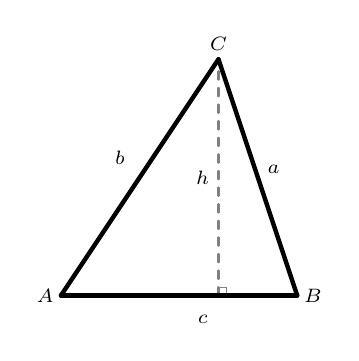
\begin{tikzpicture}[line cap=round]


    \draw [thick, dashed, gray] (2,0) -- (2,3);
    \draw [thin, gray] (2,0.1) -- (2.1,0.1);
    \draw [thin, gray] (2.1,0) -- (2.1,0.1);

	\draw [ultra thick] (0,0) -- (3,0);
	\draw [ultra thick] (3,0) -- (2,3);
	\draw [ultra thick] (0,0) -- (2,3);

 	


	\draw (2.7,1.6) node {\scriptsize{$a$}};
	\draw (0.75,1.75) node {\scriptsize{$b$}};
	\draw (1.8,-0.3) node {\scriptsize{$c$}};
	\draw (1.8,1.5) node {\scriptsize{$h$}};


	\draw (-0.2,0) node {\scriptsize{$A$}};
	\draw (3.2,0) node {\scriptsize{$B$}};
	\draw (2,3.2) node {\scriptsize{$C$}};


    \end{tikzpicture}
  \end{image}



\[    \frac{h}{b} = \sin(A)   \, \text{ and } \,    \frac{h}{a} = \sin(B)       \]



\[    h = b \sin(A)      \, \text{ and } \,    h = a \sin(B)    \]

\[     b \sin(A)  = a \sin(B)    \]


\[    \frac{\sin(A)}{a} = \frac{\sin(B)}{b}      \]




The same argument with an altitude from angle $B$ to side $b$ shows a similar relationship with angle $C$, giving us








\[    \frac{\sin(A)}{a} = \frac{\sin(B)}{b}  = \frac{\sin(C)}{c}    \]
















$\blacktriangleright$  \textbf{Obtuse Triangle}

An obtuse triangle is one with one angle greater than $90^{\circ}$. \\

We can establish the same relationship with an altitude on the outside.








\begin{image}[3in]
    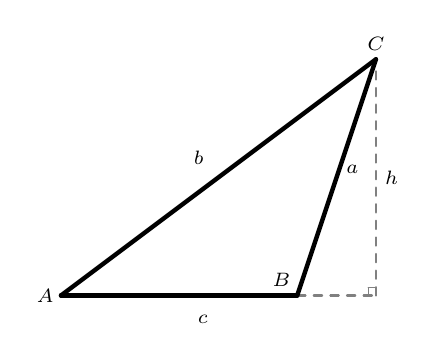
\begin{tikzpicture}[line cap=round]


    \draw [thick, dashed, gray] (4,0) -- (4,3);
    \draw [thick, dashed, gray] (3,0) -- (4,0);
    \draw [thin, gray] (4,0.1) -- (3.9,0.1);
    \draw [thin, gray] (3.9,0) -- (3.9,0.1);

	\draw [ultra thick] (0,0) -- (3,0);
	\draw [ultra thick] (3,0) -- (4,3);
	\draw [ultra thick] (0,0) -- (4,3);

 	


	\draw (3.7,1.6) node {\scriptsize{$a$}};
	\draw (1.75,1.75) node {\scriptsize{$b$}};
	\draw (1.8,-0.3) node {\scriptsize{$c$}};
	\draw (4.2,1.5) node {\scriptsize{$h$}};


	\draw (-0.2,0) node {\scriptsize{$A$}};
	\draw (2.8,0.2) node {\scriptsize{$B$}};
	\draw (4,3.2) node {\scriptsize{$C$}};


    \end{tikzpicture}
  \end{image}
















\[    \frac{h}{b} = \sin(A)   \, \text{ and } \,    \frac{h}{a} = \sin(180^{\circ} - B)  = \sin(B)      \]



\[    h = b \sin(A)      \, \text{ and } \,    h = a \sin(B)    \]

\[     b \sin(A)  = a \sin(B)    \]


\[    \frac{\sin(A)}{a} = \frac{\sin(B)}{b}      \]




The same argument could be made with angle $C$, giving us








\[    \frac{\sin(A)}{a} = \frac{\sin(B)}{b}  = \frac{\sin(C)}{c}    \]






\begin{theorem}  \textbf{\textcolor{green!50!black}{Law of Sines}} 



For any triangle with angles $A$, $B$, and $C$, and opposite sides $a$, $b$, and $c$, respectively, 


\[    \frac{\sin(A)}{a} = \frac{\sin(B)}{b}  = \frac{\sin(C)}{c}    \]


\end{theorem}





\begin{example}  General Triangles \\

Suppose we have a triangle with $A=46^{\circ}$, $B=65^{\circ}$, and $a=14$.

Figure out the other three measurements.


\begin{explanation}

$A + B + C = 46^{\circ} + 65^{\circ} + C = 180$ \\

$C = 69^{\circ}$


$\frac{\sin(46^{\circ})}{14} = \frac{\sin(65^{\circ})}{b}$

$b = \frac{14 \sin(65^{\circ})}{\sin(46^{\circ})} \approx 17.63882523$

$\frac{\sin(46^{\circ})}{14} = \frac{\sin(69^{\circ})}{c}$

$c = \frac{14 \sin(69^{\circ})}{\sin(46^{\circ})} \approx 18.16961325$

\end{explanation}


\end{example}












\begin{example}  No Triangle \\

Suppose we have a triangle with $C=55^{\circ}$, $a=4$, and $c=2$.

Figure out the other three measurements.


\begin{explanation}


$\frac{\sin(55^{\circ})}{2} = \frac{\sin(A)}{4}$

$\sin(A) = \frac{4 \sin(55^{\circ})}{2} \approx 1.638304086$

This is greater than $1$. $\sin(A)$ cannot be greater than $1$.

Therefore, there is no triangle with $C=55^{\circ}$, $a=4$, and $c=2$. 

\end{explanation}


\end{example}












\begin{example}  Two Triangles \\

Suppose we have a triangle with $A=37^{\circ}$, $a=12$, and $b=16$.

Figure out the other three measurements.


\begin{explanation}


$\frac{\sin(37^{\circ})}{12} = \frac{\sin(B)}{16}$

$\sin(B) = \frac{16 \sin(37^{\circ}}{12} \approx 0.8024200309$

There are two angles whose sine is $0.8024200309$. One in the first quadrant and one in the second quadrant. \\

Therefore, there are two triangles with $A=37^{\circ}$, $a=12$, and $b=16$. 

Using the calculator, the two angles are

\begin{itemize}
\item $B \approx SIN^{-1}(0.8024200309) \approx 53.36^{\circ}$
\item $B \approx 180^{\circ} - 53.36^{\circ} = 126.64^{\circ}$
\end{itemize}

\end{explanation}


\end{example}













\end{document}
